\begin{center} \textbf{\Large Experiments} \end{center}
To evaluate the UVAM algorithm we used the Columbia Object Image Library (COIL-100, http://www1.cs.columbia.edu/CAVE/software/softlib/coil-100.php). Therefor we extracted the 75 first objects containing the largest amount of keypoints and neglected all others. In addition, we only used objects without rotation. These objects were embedded into backgrounds taken from the McGill Calibrated Colour Image Database (http://tabby.vision.mcgill.ca/). An example test image is illustrated in Fig. 2.\\
\begin{center}
	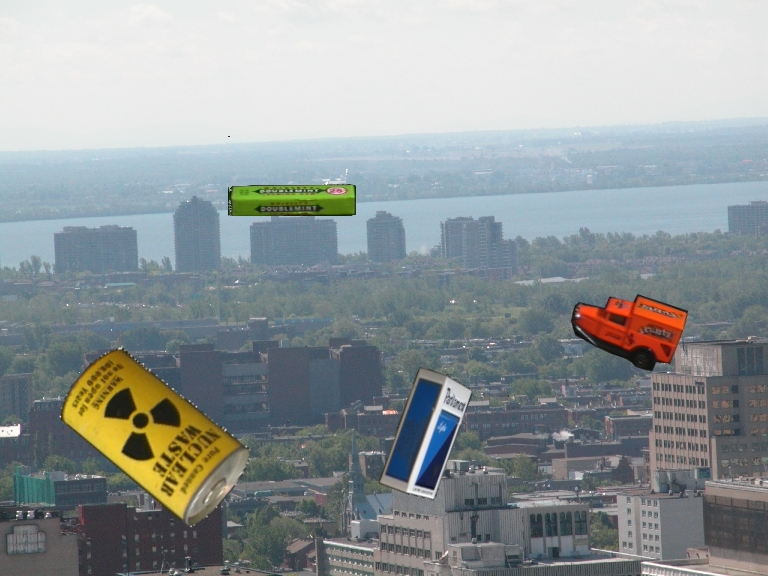
\includegraphics[scale=1.00]{img01.jpg}
	\caption{Fig. 2: An example of a test image using COIL-100 objects embedded into a background.}
	\label{fig:2}
\end{center}
To assess the performance of the UVAM algorithm and compare it, our testing procedure contained four different steps: First, we tested speed performance without the use of neither bottom-up saliency nor familiarity maps. Second, we incorporated only saliency maps into the algortihm. Third, we used only familiarity maps to test the performance. And finally, we used the actual UVAM algorithm (including both saliency and familiarity maps) to assess the speed performance of the object recognition process. 

